%!TEX root = labo.tex

\setcounter {chapter} {6} 

\chapter{Network Address Translation (NAT)\\Dynamic Host Configuration Protocol (DHCP)}

What you will learn in this lab:
\begin{itemize}
	\item How NAT (Network Address Translation) works.
	\item How DHCP (Dynamic Host Configuration Protocol) works.
	\item How DHCP works together with NAT.
\end{itemize}

\newpage
\setsession{prelab7}
\section{Prelab 7}\label{sec:prelab7}
%!TEX root = labo.tex

\subsubsection*{NAT and DHCP}
Use the following resources to prepare yourself for this lab session:
\begin{enumerate}
	\item Unix commands for NAT, DHCP: Go to the online manual pages at \url{http://manpages.ubuntu.com/}. Read the manual pages of the following commands for the operating system version "trusty 14.04 LTS":
		\begin{itemize}
			\item iptables
			\item dhclient
			\item dhcpd
			\item dhcpd.conf
			\item dhcp-options
			\item dhcpd.leases
		\end{itemize}
	\item Private IP addresses: Read RFC 1918 on address allocation in private networks \url{http://tools.ietf.org/html/rfc1918}.
	\item Network Address Translation (NAT): Read the following tutorial on NAT at \url{http://www.firewall.cx/networking-topics/network-address-translation-nat.html}.
	\item Netfilter/iptables Read about netfilter and iptables at \url{http://www.netfilter.org} and \url{http://www.thegeekstuff.com/2011/01/iptables-fundamentals/}.
	\item Dynamic Host Configuration Protocol (DHCP): Read RFC 2131 on DHCP at \url{http://tools.ietf.org/html/rfc2131}.
\end{enumerate}

\newpage
\subsection*{Prelab Questions}
\begin{questions}
	\q{1}{Explain why NAT is often mentioned as a solution to counteract the depletion of IP addresses on the global Internet? Which alternatives to NAT exist that address the scarcity of available IP addresses?}
	\q{2}{What does the following comment refer to: ``NAT destroys the ability to do host-to-host communication over the Internet``?}
\end{questions}

Explain the following terms which are used in the context of Network Address Translation:
\begin{questions}
	\q{3.a}{Static NAT}
	\q{3.b}{Dynamic NAT}
	\q{3.c}{NAT with IP overload}
	\q{3.d}{Port Address Translations e.g. IP Masquerading}
	\q{4}{Refer to RFC 1918 and list the IP address blocks that are reserved for use in private networks. Why is there a need to specify IP addresses for private networks?}	
	\q{5}{The utility netfilter and the command iptables provide support for NAT in Linux systems. Explain the relationship between the netfilter utility and the iptables command?}
\end{questions}

Describe the following terms which are used in the iptables command:
\begin{questions}
	\q{6.a}{Chain}
	\q{6.b}{Postrouting }
	\q{6.c}{Prerouting}
\end{questions}

Consider a NAT device between a private and the public network. Suppose the private network uses addresses in the range 10.0.1.0-10.0.1.255, and suppose that the interface of the NAT device to the public network has IP address 128.143.136.80.
\begin{questions}
	\q{7.a}{Write the iptables command so that the addresses in the private network are mapped to the public IP address 128.143.136.80.}
	\q{7.b}{Write an IOS command so that the addresses in the private network are mapped to the public IP address 128.143.136.80.}
\end{questions}

Answer the following questions about DHCP:
\begin{questions}
	\q{8}{Explain the meaning of the ``magic cookie'' in the DHCP protocol.}
	\q{9}{If the command \cmd{dhcpd} is issued (without arguments) on a Linux PC with multiple network interfaces, which network interfaces does the DHCP server listen on?}
\end{questions}


\newpage
\setsession{lab7}
\section{Lab 7}\label{sec:lab7}

Figure \ref{fig:lab7-part1-network} shows two private networks which are connected to a public network. Each private network is connected to the public network by a NAT device, which is either a PC or a Cisco router. On each NAT device, IP forwarding must be enabled.

\boxwarning{In the private networks in Figure \ref{fig:lab7-part1-network}, Router1 and Router3 are used to mimic hosts, i.e., they are not configured to act as IP routers.)}

\begin{figure}[ht]
	\centering
	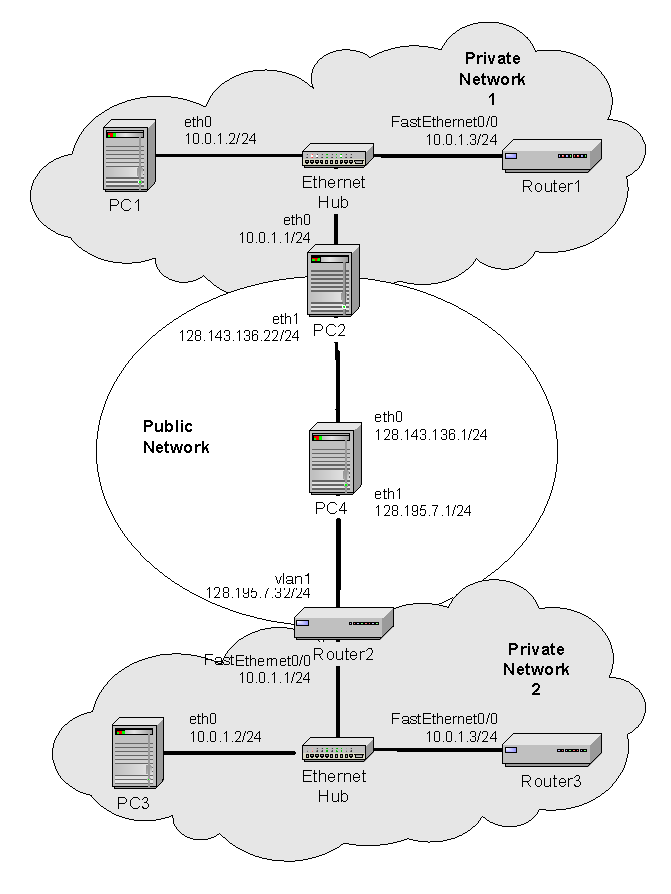
\includegraphics{graphics/lab7-part1-updated.pdf}	
	\caption{Network configuration for Part 1.}
	\label{fig:lab7-part1-network}
\end{figure}

\begin{table}[h!t]
	\centering
	\begin{tabular}{| c | c | c | c |}	
		\hline
		\textbf{Linux PC} & \textbf{IP Addresses of eth0} & \textbf{IP Addresses of eth1} & \textbf{Default Gateway} \\ \hline
		PC1 & 10.0.1.2/24 & none & 10.0.1.1 \\ 
		PC2 & 10.0.1.1/24 & 128.143.136.22/24 & 128.143.136.1 \\
		PC3 & 10.0.1.2/24 & none & 10.0.1.1 \\
		PC3 & 128.143.136.1/24 & 128.195.7.1/24 & none \\ \hline
	\end{tabular}
	\caption{IP addresses and gateways assignment of all PCs for Part 1.}
	\label{tab:lab7-part1-ip-addresses-pc}
\end{table}

\begin{itemize}
	\item In this lab, PC2 and Router2 are routers that provide the gateways between the private and the public networks. Both PC2 and Router2 are configured as NAT devices.
	\item On PC2, the kernel is built with netfilter, an extension to the Linux kernel that provides the kernel with the ability to set IP packet filters, including NAT functions. On Router2, you will use Cisco IOS commands to configure NAT rules.
	\item PC4 runs as an IP router. (We use a Linux PC instead of a Cisco Router so that wireshark can be used to capture traffic on the public network).
	\item The assignment of IP addresses and default gateways for all PCs and routers are shown in Table1 and Table 2.
	\item The console port of Router1 is connected to a serial port of PC1, the console port of Router2 is connected to a serial port of PC2, and the console port of Router3 is connected to a serial port of PC3.
\end{itemize}

\begin{table}[h!t]
	\centering
	\begin{tabular}{| c | c | c | c | c |}	
		\hline
		\textbf{Linux PC} & \textbf{IP Addresses of FA0/0} & \textbf{IP Addresses of vlan1} & \textbf{Default Gateway} & \textbf{Connected PC} \\ \hline
		Router1 & 10.0.1.3/24 & none & 10.0.1.1 & PC1 \\ 
		Router2 & 10.0.1.1/24 & 128.195.7.32/24 & 128.195.7.1 & PC2 \\
		Router3 & 10.0.1.3/24 & none & 10.0.1.1 & PC3\\ \hline
	\end{tabular}
	\caption{IP addresses and gateways assignment of all routers for Part1.}
	\label{tab:lab7-part1-ip-addresses-routers}
\end{table}

\newpage
\subsection{NAT (Network Address Translation)}

NAT (Network Address Translation) refers to a function that replaces the IP addresses (and possibly the port numbers) of IP datagrams. NAT is run on routers that connect private networks to the public Internet, to replace the IP address-port pair of an IP packet with another IP address-port pair. Generally, the operations of NAT are specified in terms of a set of rules which determines how IP addresses are to be replaced.

Often, a NAT device is referred to as a NAT box. One of the reasons for using NAT is that it conserves IP addresses. NAT allows hosts in a private network to share public IP addresses, or to limit the use of public IP addresses to a small number of hosts in the private network.

Private networks may have IP addresses that are non-Internet routable, as specified in RFC 1918. This means that the Internet routers do not have entries in their routing tables for these addresses.

In the network in Figure \ref{fig:lab7-part1-network}, both PC2 and Router2 will be configured as NAT devices. With NAT, the hosts in the private networks can access the public network, i.e., they are able to reach the addresses on the 128.143.136.0/24 and 128.195.7.0/24 networks.

\subsubsection{Exercise 1-a: Network Setup}
Configure the network in Figure \ref{fig:lab7-part1-network} with the IP address configuration shown in Table \ref{tab:lab7-part1-ip-addresses-pc} and Table \ref{tab:lab7-part1-ip-addresses-routers}. The following commands review the steps involved in the configuration.
\begin{enumerate}
	\item On the Linux PCs, use \cmd{ifconfig} to configure the IP address of the interfaces. Add a default gateway on each PC with the command (shown for PC1):
		\begin{cmdblock}
	PC1% route add default gw gateway_address
	\end{cmdblock}
	\item IP forwarding must be enabled on PC2 and PC4.
	\item Use a serial cable to connect a serial port of a PC to the console port of a router. Use the \cmd{minicom} command to access the routers.
	\item Configure the IP addresses of interfaces \iface{Fa/0} and \iface{vlan1} on the routers, and set the default gateways as shown in Table \ref{tab:lab7-part1-ip-addresses-routers}. Below is the sample configuration for Router2.
		\begin{cmdblock}
	Router2> enable
	Password: <enable secret>
	Router2# configure terminal
	Router2(config)# no ip routing
	Router2(config)# ip routing
	Router2(config)#ip route 0.0.0.0 0.0.0.0 128.195.7.1
	Router2(config)# interface FastEthernet0/0 
	Router2(config-if)# no shutdown
	Router2(config-if)# ip address 10.0.1.1 255.255.255.0 
	Router2(config-if)# interface FastEthernet0/1 
	Router2(config-if)# no shutdown
	Router2(config-if)# interface vlan1 
	Router2(config-if)# no shutdown
	Router2(config-if)# ip address 128.195.7.32 255.255.255.0
	Router2(config-if)# end
		\end{cmdblock}
		The following commands sets 128.195.7.1 as the default gateway of Router2.
		\begin{cmdblock}
	Router2(config)# ip route 0.0.0.0 0.0.0.0 128.195.7.1
		\end{cmdblock}
\end{enumerate}

After completing the set up of the configuration you should be able to issue successful intra network ping commands i.e., between hosts in the private network, and between hosts in the public network. However, ping commands across a private/public network boundary are not successful.

\subsubsection{Exercise 1-b: Configuration of NAT on a Cisco Router}
\boxwarning{You will use Wireshark in this exercise. Do not forget to append the binary dump (pcap format) to your lab report}
A Cisco router can be set up to run as a NAT device.

\boxinfo {In Cisco IOS, the private network is referred to as ``inside'' and the public network is referred to as ``outside''. An IP address that is seen by hosts on the inside is called a local address, and an IP address that is seen by hosts on the outside is called a global address. There are four different types of addresses:
\begin{itemize}
	\item An inside local address is an address in the private network that is not visible in the public network.
	\item An inside global address can be used in the public network for devices in the private network.
	\item An outside global address is an address in the public network that is not made known in the private network.
	\item An outside local address is used by devices in the private network to addresses in the public network.
\end{itemize}
Using this terminology, a NAT device translates inside local addresses to outside global addresses and outside global addresses to inside local addresses.
}

\begin{enumerate}
	\item Modify the NAT table of Router2: Use the following commands to set up Router2 as a NAT device.
		\begin{itemize}
			\item A NAT rule is added so that the private IP address of PC3, 10.0.1.2, is translated to the public address 200.0.0.2.
				The IOS commands are as follows:
				\begin{cmdblock}
	Router2> enable
	Password: <enable secret>
	Router2# show ip nat translations
	Router2# configure terminal
	Router2(config)# interface FastEthernet0/0
	Router2(config-if)# ip nat inside
	Router2(config-if)# interface vlan1
	Router2(config-if)# ip nat outside
	Router2(config-if)# exit
	Router2(config)# ip nat inside source static 10.0.1.2 200.0.0.2 
	Router2(config)# end
	Router2# show ip nat translations
				\end{cmdblock}
			\item After the above rule has been entered, display the content of the NAT table and save it to a file.
				The commands used above are explained below:
				\begin{itemize}
					\item Displays the content of the NAT table:
						\begin{cmdblock}
	Router2# show ip nat translations
						\end{cmdblock}
					\item Specifies that interface \iface{FastEthernet0/0} is connected to the private network.
						\begin{cmdblock}
	Router2(config)# interface FastEthernet0/0
	Router2(config-if)# ip nat inside
						\end{cmdblock}
					\item Specifies that interface \iface{vlan1} is connected to the public network.
						\begin{cmdblock}
	Router2(config-if) #interface vlan1
	Router2(config-if)# ip nat outside
						\end{cmdblock}
					\item Adds a rule so that the private address 10.0.1.2 is mapped to the public address 200.0.0.2
						\begin{cmdblock}
	Router2(config)# ip nat inside source static 10.0.1.2 200.0.0.2
						\end{cmdblock}
				\end{itemize}
			\end{itemize}
		\boxinfo {``Dynamic NAT'' is an alternative to the static NAT table entries used in this exercise. With dynamic NAT, a pool of global addresses is specified at the NAT device. Addresses from the pool are dynamically mapped to the private addresses whenever there is a demand for a new address.}
	\item Update routing tables: Add static routing entries to the routing table of PC4, so that traffic with destination IP address 200.0.0.0/24 is forwarded to Router2.
	\item Observe traffic at a NAT device: To observe the IP address translation, issue ping commands between machines in the public and private network. Use Wireshark to capture packets on the private and public interfaces of Router2.
		\begin{itemize}	
			\item Start an Wireshark session on PC3 to capture the traffic from Router2 on the private network.
			\item Start an Wireshark session on interface \iface{eth1} of PC4 to capture the traffic from Router2 on the public network.
			\item Issue the following ping commands: 
				On PC3:
				\begin{cmdblock}
	PC3% ping -c 3 10.0.1.3
	PC3% ping -c 3 128.143.136.1
				\end{cmdblock}
				On Router3:
				\begin{cmdblock}
	Router3# ping 10.0.1.2
	Router3# ping 128.143.136.1
				\end{cmdblock}
				On PC4:
				\begin{cmdblock}
	PC4% ping -c 3 10.0.1.2 
	PC4% ping -c 3 200.0.0.2
				\end{cmdblock}
			\item Save the Wireshark data to files. Observe which ping commands succeed.
		\end{itemize}
	\item Add additional NAT table entries: Add NAT rules to Router2, so that Router2 and Router3 (on interface \iface{Etherenet0/0}) are addressable from the public network. The private and public addresses are given in Table \ref{tab:lab7-nat-router2-router3}.
		\begin{table}[h!t]
			\centering
			\begin{tabular}{| c | c | c |}	
				\hline
				\textbf{Linux PC} & \textbf{Inside local address} & \textbf{Outside local address}  \\ \hline
				Router2 & 10.0.1.1/24 & 200.0.0.1 \\ 
				Router3 & 10.0.1.3/24 & 200.0.0.3 \\ \hline
			\end{tabular}
			\caption{Private and public addresses of Router2 and Router3.}
			\label{tab:lab7-nat-router2-router3}
		\end{table}
\end {enumerate}

\begin{questions}
	\q{1.B.a}{Include the NAT table of Router2 and provide an explanation of the columns of the table.}
	\q{1.B.b}{For each of the ping commands above, provide an explanation why the command succeeds or fails.}
	\q{1.B.c}{Include the IP source address and IP destination address from the IP header data of an ICMP request and the corresponding ICMP reply packet before and after it passes through Router2.}
\end{questions}
	
\subsubsection{Exercise 1-c: IP Masquerading with a Linux PC}
\boxwarning{You will use Wireshark in this exercise. Do not forget to append the binary dump (pcap format) to your lab report}
In this exercise, we consider a special use of NAT that allows multiple private IP addresses to be mapped to a single public IP address. This use of NAT is called IP masquerading, port address translation (PAT) or Network Address and Port Translation (NAPT). Here, the private network has only a single public IP address, but has multiple hosts in the private network. IP Masquerading modifies the port number of packets so that the single public IP address can be overloaded.

In this exercise, PC2 will be configured to perform IP masquerading. The Linux kernel on all PCs has been built with netfilter, which adds the ability to set IP packet filters in a Linux system. IP packet filters are used to add firewalls as well as NAT functionality to a system. The \cmd{iptables} command is used to set up, maintain, and inspect IP packet filter rules to a Linux kernel.

\boxinfo {On a Linux system, the configuration of NAT manipulates a set of rules of the netfilter utility, called NAT table. The rules in the NAT table are grouped in so- called chains. Two of the built-in chains are called \texttt{PREROUTING} and \texttt{POSTROUTING}:
	\begin{description}
		\item[\texttt{PREROUTING}] \hfill \\
			The rules in this chain are applied to incoming datagrams.
		\item[\texttt{POSTROUTING}] \hfill \\
			The rules in this chain are applied to outgoing datagrams. The main rule is SNAT (Source Network Address Translation), which specifies how the source address of an outgoing IP datagram should be modified.
	\end{description}
}

Commands that manipulate the NAT table start with
\begin{cmdblock}
	PC2% iptables -t nat
\end{cmdblock}

\boxinfo {The following are some of the most important commands that manipulate the NAT table:
	\begin{description}
		\item[\texttt{iptables -t nat -L}] \hfill \\
			Displays all rules in the NAT table
		\item[\texttt{iptables -t nat -L}] \hfill \\
			Deletes the first rule in the \texttt{POSTROUTING} chain of the NAT table
		\item[\texttt{iptables -t nat -F}] \hfill \\
			Deletes all entries in (``flushes'') the NAT table
		\item[\texttt{iptables -t nat -A POSTROUTING -j SNAT -{}-to IPAddr -s PrivateIPAddr/netmask}] \hfill \\
			Adds the following rule to the \texttt{POSTROUTING} chain of the NAT table: ``In IP datagrams that go to the public network, the IP source address PrivateIPAddr/netmask is changed to IPAddr''.\\
			Example: The source address of outgoing IP datagrams that match ``10.0.1.0/24'' is changed to 128.195.7.32.\\
			\cmd{iptables -t nat -A POSTROUTING -j SNAT -{}-to 128.195.7.32 -s 10.0.1.0/24}
	\end{description}
}

\begin{enumerate}
	\item Modify the NAT table of PC2: On PC2, add a rule to the NAT table so that the IP source address of all outgoing IP datagrams are set to IP address 128.143.136.22. Display the content of the NAT table and save it to a file.
	\item Observe traffic at a NAT device:
		\begin{itemize}
			\item To observe the IP address translation, capture packets on both interfaces of PC2 that are between the private networks and the Internet. On PC2, run Wireshark on both \iface{eth0} and \iface{eth1}.
			\item Establish a set of Telnet session and login to remote machines, using the following \cmd{telnet} commands:
				On PC1:
				\begin{cmdblock}
	PC1% telnet 10.0.1.3
	PC1% telnet 128.143.136.1
				\end{cmdblock}
				On Router1:
				\begin{cmdblock}
	Router1# telnet 10.0.1.2
	Router1# telnet 128.143.136.1
				\end{cmdblock}
				On PC4:
				\begin{cmdblock}
	PC4% telnet 10.0.1.2
				\end{cmdblock}
			\item Save the Wireshark data to files. Observe which Telnet commands succeed.
			\item For the successful Telnet sessions, observe how the IP addresses and port numbers are mapped.
		\end{itemize}
	\item Observe mapping of ICMP packets: The ping command sends out ICMP Echo Request messages and receives ICMP Echo Reply messages. Since ICMP messages do not contain a port number, it is not entirely obvious how a NAT device that performs IP masquerading can direct ICMP Echo Reply messages that return from the public network to the private network. In this exercise, you will explore how a NAT device handles ICMP messages.
		\begin{itemize}
			\item On PC2, run Wireshark on both \iface{eth0} and \iface{eth1}. Use the appropriate filters to capture the traffic generated by ping commands.
			\item Issue the following ping commands:
				On PC1:
				\begin{cmdblock}
	PC1% ping -c 3 10.0.1.3
	PC1% ping -c 3 128.143.136.1
				\end{cmdblock}
				On Router1:
				\begin{cmdblock}
	Router1# ping 10.0.1.2
	Router1# ping 128.143.136.1
				\end{cmdblock}
				On PC4:
				\begin{cmdblock}
	PC4% ping -c 3 10.0.1.2
				\end{cmdblock}
			\item Save the Wireshark output and the output of ping commands into files.
		\end{itemize}
\end{enumerate}

\begin{questions}
	\q{1.C.a}{For each of the \cmd{telnet} and \cmd{ping} commands above, provide an explanation why a command succeeds or fails.}
	\q{1.C.b}{For each successful telnet session, include the IP header data of an outgoing and an incoming packet header (with respect to the private network).}
	\q{1.C.c}{For each successful ping command, include the IP header data of an outgoing ICMP Request message and an incoming ICMP reply message (with respect to the private network).}
	\q{1.C.d}{How does PC know that a packet coming from the public network is destined to a host in the private network?}
	\q{1.C.e}{Explain the steps performed by the kernel during IP address translation.}
\end{questions}

\subsubsection{Exercise 1-d: NAT and FTP}
\boxwarning{You will use Wireshark in this exercise. Do not forget to append the binary dump (pcap format) to your lab report}

NAT can create problems for applications, which carry the IP addresses in the payload of an IP datagram. An example of such an application is the file transfer program (FTP).

In this exercise, you establish an FTP connection from PC3 in the private network to PC2 in the public network, and observe how the FTP application works with NAT.

\begin{enumerate}
	\item Start Wireshark on interface \iface{eth0} of PC4 and on interface \iface{eth0} of PC3.
	\item FTP session between two hosts in the public network:
		\begin {itemize}
			\item Start the FTP server on PC2 by typing
				\begin{cmdblock}
	PC2% service vsftpd start
				\end{cmdblock}
			\item Start an FTP connection from PC4 to PC2 (the -d option prints out debug messages).
				\begin{cmdblock}
	PC4% cd /root/labdata
	PC4% ftp -d 128.143.136.22
				\end{cmdblock}
				Login with user name ``root'' and enter the root password.
			\item Download a file from the FTP server.
				\begin{cmdblock}
	ftp> get fname
				\end{cmdblock}
				where \path{fname} is a file on the remote server. (You can use the command ls to obtain a list of all files in the remote directory.)
			\item Use the traffic captured by Wireshark to determine where the payload of FTP data carries information on IP addresses.
			\item Save the Wireshark output and the FTP debug information output into files.
		\end{itemize}
	\item FTP session from a private to the public network:
		\begin{itemize}
			\item Use the same commands as previously to download a file from PC2 to PC3
				\begin{cmdblock}
	PC3% ftp -d 128.143.136.22
				\end{cmdblock}
				Is the FTP session establishment successful?
			\item Save the traffic captured by wireshark and save the FTP debug information output. Make sure that you save enough data to answer the lab report questions.
		\end{itemize}
\end{enumerate}

\begin{questions}
	\q{1.D.a}{Use the captured data to explain the outcome of the FTP experiment. In particular, if the file was successfully downloaded, explain how the problem of sending the IP address as part of the data payload of the IP packet is solved.}
	\q{1.D.b}{How can NAT be used to spoof a host address? How can you prevent this?}
\end{questions}

\newpage
\subsection{Dynamic Host Configuration Protocol (DHCP)}

The Dynamic Host Configuration Protocol (DHCP) can be used to dynamically set and change configuration parameters of Internet hosts, including IP address, subnet mask, default router, and DNS server. DHCP is based on a client-server model. DHCP clients send requests to a DHCP server and the server responds with an allocation of IP addresses and other configuration parameters.

In this part of the lab, you will also learn about DHCP relay agents. When the DHCP client and DHCP server are not on the same IP network, DHCP relay agents can act as routers of DHCP messages. A DHCP relay agent can forward DHCP requests from a DHCP client to a DHCP server and it can forward the reply messages from the DHCP server to the DHCP client.

The network configuration for Part 2 is shown in Figure \ref{fig:lab7-part2}. PC1, PC3, and PC4 are set up as DHCP clients, and initially do not have IP addresses. PC2 is configured as a DHCP server, which listens for DHCP requests on all of its interfaces and transmits network configuration parameters. Router1 acts as a DHCP relay agent, which forwards DHCP messages between different IP networks.

Table \ref{tab:lab7-part2-ip-addresses-pc} lists the range of addresses that are associated at the DHCP server PC2 with each IP network.

\begin{figure}[h!t]
	\centering
	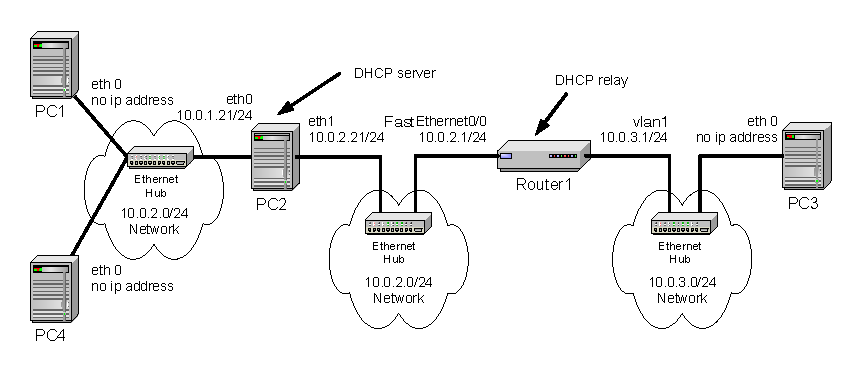
\includegraphics{graphics/lab7-part2-updated.pdf}	
	\caption{Network configuration for Part 2.}
	\label{fig:lab7-part2}
\end{figure}

\begin{table}[h!t]
	\centering
	\begin{tabular}{| c | c | c | c |}	
		\hline
		\textbf{Linux PC} & \textbf{IP Addresses of eth0} & \textbf{IP Addresses of eth1} & \textbf{Default Gateway} \\ \hline
		PC1 & none & none & none \\ 
		PC2 & 10.0.1.21/24 & 10.0.2.21/24 & 10.0.2.1 \\
		PC3 & none & none & none \\ 
		PC3 & none & none & none \\ \hline
	\end{tabular}
	\caption{Configuration of the PCs in Part 2.}
	\label{tab:lab7-part2-ip-addresses-pc}
\end{table}

\begin{table}[h!t]
	\centering
	\begin{tabular}{| c | c | c | c | c |}	
		\hline
		\textbf{Linux PC} & \textbf{IP Addresses of eth0} & \textbf{IP Addresses of eth1} & \textbf{Default Gateway} & \textbf{Connected PC} \\ \hline
Router1 & 10.0.2.1/24 & 10.0.3.1/24 & 10.0.2.21 & PC1 \\ \hline
	\end{tabular}
	\caption{Configuration of the Routers in Part 2.}
	\label{tab:lab7-part2-ip-addresses-routers}
\end{table}

\begin{table}[h!t]
	\centering
	\begin{tabular}{| c | c | c | c | c |}	
		\hline
		\textbf{Subnet} & \textbf{Range of Addresses} & \textbf{Default Router} \\ \hline
		10.0.1.0/24 & 10.0.1.2 to 10.0.1.10 & 10.0.1.21 \\ 
		10.0.3.0/24 & 10.0.3.2 to 10.0.3.10 & 10.0.3.1 \\ \hline
	\end{tabular}
	\caption{DHCP server configuration.}
	\label{tab:lab7-part2-dhcp}
\end{table}

\subsubsection{Exercise 2-a: Network Setup}
\begin{enumerate}
	\item We strongly recommend that you reboot the PCs and the routers before you proceed. Don't forget to save your files on a USB stick or online before rebooting.
	\item Set up the network topology as shown in Figure \ref{fig:lab7-part2}. Configure the IP addresses of the PCs and Router1 as shown in Table \ref{tab:lab7-part2-ip-addresses-pc} and Table {tab:lab7-part2-ip-addresses-routers}.
	\item It is important that PC1, PC3 and PC4 do not have a default route and do not have an IP address associated with their respective interface eth0.
\end{enumerate}

Review the routing table and the interface configuration. On PC1, this is done with the commands:

\begin{cmdblock}
	PC1% netstat -rn
	PC1% ifconfig -a
\end{cmdblock}

In Linux, routing tables display the default route as an entry with destination 0.0.0.0. If the routing table shows a default route, you can delete this and all other routing table entries by setting the IP address to 0.0.0.0. This is done with the following command:

\begin{cmdblock}
	PC1% ifconfig eth0 0.0.0.0 up
\end{cmdblock}

\subsubsection{Exercise 2-b: Configuring and starting a DHCP server}
On a Linux system, a DHCP server is started with the command \cmd{dhcpd}. The DHCP server reads the configuration file \path{/etc/dhcpd.conf}. The configuration file contains information on available IP addresses, and other configuration information. The following is an example of a configuration file for a DCHP server:

\begin{cmdblock}
	#dhcpd.conf file
	default-lease-time 600;

	subnet 10.0.1.0 netmask 255.255.255.0 {
		range 10.0.1.10 10.0.1.100; 
		option routers 10.0.1.1; 
		default-lease-time 120;
	}
	subnet 10.0.2.0 netmask 255.255.255.0 {
		range 10.0.2.101 10.0.2.200; 
	}

	subnet 10.0.3.0 netmask 255.255.255.0 { 
		range 10.0.3.6 10.0.3.10;
	}
\end{cmdblock}

The DHCP client is assigned an IP address for a period of time that is known as a lease. The above configuration file assigns IP addresses for a lease time of 600 seconds (default-lease- time). For requests on network 10.0.1.0/24, the DHCP server assigns IP addresses in the range 10.0.1.10 - 10.0.1.100, assigns 10.0.1.1 as the default gateway, and limits the lease of addresses to 120 seconds, thus, overruling the global limit of 600 seconds. For requests on network 10.0.2.0/24, the server assigns IP addresses in the range 10.0.2.101- 10.0.2.200.

\begin{enumerate}
	\item Set the DHCP configuration file: On PC2, set up the configuration file so that IP addresses are assigned as follows. On network 10.0.1.0/24, IP addresses are assigned in the range 10.0.1.2-10.0.1.10 with default gateway 10.0.1.21. On network 10.0.3.0/24, IP addresses are assigned in the range 10.0.3.2-10.0.3.10 with default gateway 10.0.3.1.
Note that these assignments are similar to, but not identical with the configuration file shown above.
	\item Start the DHCP server: On PC2, start the DHCP server by typing 
		\begin{cmdblock}
	PC2% dhcpd
		\end{cmdblock}
		The DHCP server daemon listens for requests from DHCP clients on all its interfaces. In Linux, the DHCP server must be restarted each time the configuration file is modified. Since only one DHCP server can run at a time, you may need to terminate the current DHCP server process.
\end{enumerate}

\subsubsection{Exercise 2-c: Starting a DHCP client}
\boxwarning{You will use Wireshark in this exercise. Do not forget to append the binary dump (pcap format) to your lab report}

The following steps start a DHCP client on PC1.
\begin{enumerate}
	\item On PC1, perform the following functions:
		\begin{itemize}
			\item Ensure that no default router entry exists in the routing table.
			\item A Linux DHCP client caches information from previous uses of DHCP. The cached information is stored in :
				\begin{cmdblock}
	/var/lib/dhcp3/
				\end{cmdblock}
				Since this cached information may interfere with your work, delete the lease files related to dhclient, if they exist:
				\begin{cmdblock}
	rm /var/lib/dhcp3/dhclient*
				\end{cmdblock}
			\item Start Wireshark on interface \iface{eth0} of PC2. (Set the display filter to ``bootp.dhcp'' so that only DHCP traffic is displayed in the window.)
		\end{itemize}
	\item Start a DHCP client with the command
		\begin{cmdblock}
	PC1% dhclient eth0
		\end{cmdblock}
\end{enumerate}

Save the data that is captured by Wireshark to a file. Save enough data to answer the following questions from the captured traffic:

\begin{questions}
	\q{2.C.2.a}{Which IP address is assigned to PC1?}
	\q{2.C.2.b}{	Observe the source and destination IP addresses of the packets that are sent between DHCP client and DHCP server.}
	\q{2.C.2.c}{How is it possible that a host can send and receive DHCP packets, even though it does not have an IP address?}
	\q{2.C.2.d}{Do you observe any ARP packets? If so, explain the function of the ARP in this context.}
	\q{2.C.2.e}{Observe and interpret the output of the DHCP packets. You should see the following packet types: DHCP Discover, DHCP Offer, DHCP Request, DHCP ACK.}
	\q{2.C.2.f}{Identify and interpret all option fields in the DHCP packet types that you observe.}
\end{questions}

\begin{enumerate}
	\item Renewing leases of IP addresses: The DHCP client is assigned an IP address for a limited period of time, which is called a lease. The maximum time of a lease is specified in the \path{dhcpd.conf} file. Information on current leases is stored at both the client side and the server side.
		\begin{itemize}
			\item In Linux, information on the current leases is stored in the following files \path{/etc/dhcpd.leases} at the DHCP server and \path{/var/lib/dhcp3/dhclient-eth0.lease} at the DHCP client (note that the latter name may differ).
			\item To interpret the content of the files, refer to the manual pages of dhcpd.conf, dhcp-options, and dhcpd.leases.
			\item Save the files that contain the information on current leases.
			\item Observe how a DHCP client renews a lease and save the captured traffic to a file.
				\begin{itemize}
					\item What type of DHCP message can be observed?
					\item How long does a DHCP client wait until it attempts to renew its lease?
				\end{itemize}
			\item Stop the process that runs the DHCP server by terminating the process \cmd{dhcpd} with the command
				\begin{cmdblock}
	PC2% pkill dhcpd
				\end{cmdblock}
				Observe what the DHCP client does when it cannot reach the DHCP server. Use the command \cmd{ifconfig -a} to see how long the DHCP client waits until it releases the leased IP address.
			\item Restart the DHCP server process by typing
				\begin{cmdblock}
	PC2% dhcpd
				\end{cmdblock}
		\end{itemize}
	\item Starting more DHCP clients: Repeat the instructions in Step 2 and start DHCP clients on PC3 and PC4.
\end{enumerate}

\begin{questions}
	\q{2.C.4.a}{The expected outcome is that PC4 receives an IP address, but that PC3 is not successful. Why is the negative outcome for PC3 expected?}
	\q{2.C.4.b}{Compare the IP addresses assigned to PC1 and PC4. Is there a specific order in which IP addresses are assigned by the DHCP server?}
	\q{2.C.a}{Use a figure to explain the packets that were exchanged by the DHCP client and the DHCP server as part of the process of acquiring an IP address.}
	\q{2.C.b}{Explain the entries in the lease file. How is the content of the lease file used when a DHCP server cannot contact the DHCP server?}
	\q{2.C.c}{In most client-server application, the port number of a server is a well-known number (e.g., an FTP server uses port number 21, the telnet server uses port number 23, etc.), while the client uses a currently available (ephemeral) port number. DHCP is different. Here, both the client and the server use a well-known port: UDP port 67 for the DHCP server, and UDP port 68 for the DHCP client. Refer to RFC 2131 and provide an explanation for this protocol design choice.}
	\q{2.C.d}{Another protocol that can be used to assign IP addresses is the Reverse ARP (RARP) protocol. Compare the services provided by RARP and DHCP.}
\end{questions}
	
\subsubsection{Exercise 2-d: DHCP relay agent}
\boxwarning{You will use Wireshark in this exercise. Do not forget to append the binary dump (pcap format) to your lab report}

A DHCP relay agent can forward DHCP packets when both the DHCP server and the DHCP client are not on the same network. Note that the role of a DHCP relay agent is not entirely trivial, since it acts as a router for a host that does not have an IP address. Here you explore, how packets from the client reach the server on another network, and how the response from the server reaches the DHCP client.
The DHCP server is configured to allocate addresses as shown in Table \ref{tab:lab7-part2-dhcp}

\begin{enumerate}
	\item Setting up a Cisco router as a DHCP relay agent: The following commands set up Router1 as a DHCP relay agent. In essence, Router1 is configured to forward UDP packets.
		Start the DHCP relay agent on Router1 as follows:
		\begin{cmdblock}
	Router> enable Password: <enable secret>
	Router1# configure terminal
	Router1(config)
	Router1(config) ip forward-protocol udp 
	Router1(config) interface vlan1 
	Router1(config-if) ip helper-address 10.0.2.21 
	Router1(config-if) end
		\end{cmdblock}
		\boxinfo{The following explains some of the above used commands:
			\begin{description}
				\item[\texttt{ip forward-protocol udp}] \hfill \\
					Enables UDP packet forwarding.
				\item[\texttt{ip helper-address 10.0.2.21}] \hfill \\
					The DHCP request packets received on vlan1 will be forwarded to the DHCP server with address 10.0.2.21.
			\end{description}
		}
	\item Start Wireshark on PC2 and PC3.
	\item Make sure that the DHCP server is running on PC2. If necessary, start a new DHCP
server.
	\item Start a DHCP client on PC3 with
		\begin{cmdblock}
	PC3% dhclient eth0
		\end{cmdblock}
	\item Verify that an IP address has been assigned to PC3. According to the configuration file, the DHCP configuration on network 10.0.2.0/24 does not set a default router. Verify that this is correct, by inspecting the routing table.
\end{enumerate}

\begin{questions}
	\q{2.D.a}{Include the Wireshark data of the first three DHCP packets that are exchanged between PC3 and PC2.}
	\q{2.D.6.a}{Does the DHCP relay server modify DHCP packets or the IP header? If so, what are the modifications?}
	\q{2.D.6.b}{How does the relay agent redirect the replies from the DHCP server? Does it broadcast them or unicast them to the DHCP client?}
	\q{2.D.6.c}{Is there a difference in the response of the DHCP server as compared to the DHCP configuration of PC1? If so, explain the difference.}
	\q{2.D.6.d}{How does the DHCP server (PC2) know on which network PC3 is located, when it receives the DHCP request?}
	\q{2.D.6.e}{What is the destination IP address of the first DHCP packet that the DHCP server sends to PC3?}
	\q{2.D.c}{What happens if a network has multiple DHCP servers?}
\end{questions}

\newpage
\section{Combining NAT and DHCP}

Figure \ref{fig:lab7-part3} shows a network configuration which can be found in many SOHO (small office, home office) networks.

\begin{itemize}
	\item The SOHO network is a private network with multiple hosts (PC1 and PC4) and one IP router (PC2).
	\item The IP router of the SOHO network (SOHO router) provides access to the public Internet by connecting to a router of an Internet service provider. The SOHO router obtains a single IP address on the "public" interface of the SOHO network via DHCP from a DHCP server (PC3) of the Internet service provider.
	\item The SOHO router works as a DHCP server and NAT server for the hosts in the SOHO network.
\end{itemize}

In this network setup, all SOHO hosts can share a single public IP address, which is dynamically assigned by the Internet service provider. Furthermore, the SOHO network requires minimal IP configuration. The hosts in the SOHO network obtain their IP address from the SOHO router. The SOHO router obtains its (public) IP address from the Internet service provider.

Your task is to setup the entire SOHO network, including the router and the DHCP server of the Internet service provider.

\begin{figure}[h!t]
	\centering
	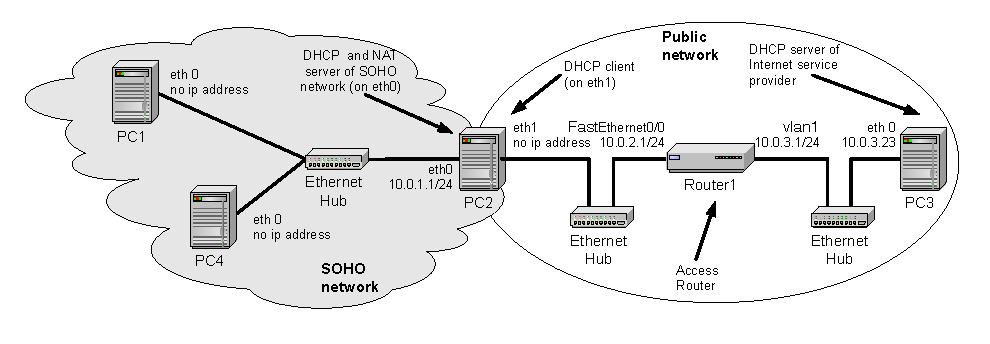
\includegraphics{graphics/lab7-part3-updated.pdf}	
	\caption{Network configuration for Part 3.}
	\label{fig:lab7-part3}
\end{figure}

\subsection{Exercise 3:}
\boxwarning{You will use Wireshark in this exercise. Do not forget to append the binary dump (pcap format) to your lab report}

The network configuration is shown as Figure \ref{fig:lab7-part3}. (The connections of the cables are identical to Figure \ref{fig:lab7-part2}). To reset the configuration of all machines, we recommend rebooting the PCs and the router.

\begin{enumerate}
	\item DHCP Server: PC3 is the DHCP server of the Internet service provider.
		\begin{itemize}
			\item Configure PC3 with IP address 10.0.3.23/24 on interface \iface{eth0} and with default gateway 10.0.3.1.
			\item Configure and start a DHCP server on PC3. On PC3, set up the configuration file so that IP addresses in the range 10.0.2.2-10.0.2.10 are assigned for requests on network 10.0.2.0/24, and addresses in the range 10.0.3.2-10.0.3.10 are assigned for requests on network 10.0.3.0/24.
		\end{itemize}
	\item Router and DHCP relay agent: Router1 is the IP router to which the SOHO network sends its external traffic. Also, Router1 is a DHCP relay agent.
		\begin{itemize}
			\item Configure Router1 with IP addresses 10.0.2.1/24 on interface \iface{FastEthernet0/0} and 10.0.3.1/24 on interface \iface{vlan1}.
			\item The routing table of Router1 should reflect that all traffic to network 10.0.2.0/24 is sent on interface \iface{FastEthernet0/0}, and all other traffic is sent on interface \iface{vlan1}.
			\item Configure Router1 as a DHCP relay agent, so that requests from DHCP client PC2 reach DHCP server PC3.
		\end{itemize}
	\item SOHO Router: PC2 is the SOHO router.
		\begin{itemize}
			\item Set up PC2 so that it is a DHCP client on interface \iface{eth1}.
			\item Set up PC2 as an IP router. That is, IP forwarding must be enabled. The routing table entries must reflect that traffic to network 10.0.1.0/24 must be routed on interface \iface{eth0}, and all other traffic must be sent to Router1 at 10.0.2.1.
			\item Configure PC2 as DHCP server on interface \iface{eth0} for addresses in the range 0.0.1.2 - 10.0.1.10. Execute the following command to start a DHCP server process on PC2:
				\begin{cmdblock}
	PC2% dhcpd eth0
				\end{cmdblock}
			\item Start a NAT server on PC2 and set up a NAT table, which maps packets from the SOHO network with source IP address from network 10.0.1.0/24 to the IP address of interface \iface{eth1}, PC2 obtained through DHCP protocol from PC3. The command for adding a rule that will achieve this is:
				\begin{cmdblock}
	iptables -t nat -A POSTROUTING -j MASQUERADE -o eth1 -s 10.0.1.0/24
				\end{cmdblock}
		\end{itemize}
	\item Hosts in PCs: PC1 and PC4 are hosts in the SOHO network.
		\begin{itemize}
			\item Set up PC1 and PC4 as DHCP clients on interfaces \iface{eth0}.
		\end{itemize}
	\item Collecting the results:
		\begin{itemize}
			\item Display the routing tables from all PCs with \cmd{netstat -rn}, and the IP configuration with \cmd{ifconfig -a}, and save the results.
			\item What are the IP addresses assigned to PC1 and PC4? How are the IP addresses mapped to the public IP address defined on the NAT server PC2?
			\item Display and save the NAT table of PC2.
			\item Start Wireshark on PC1 (\iface{eth0}), PC2 (\iface{eth1}), and PC3 (\iface{eth0}).
			\item Issue a \cmd{ping} command from PC1 to PC3:
				\begin{cmdblock}
	PC1% ping -c 5 10.0.3.23
				\end{cmdblock}
			\item Save the traffic captured by Wireshark on one of the PCs to a file.
		\end{itemize}
\end{enumerate}

\begin{questions}
	\q{3.a}{Include the Wireshark data from the first ICMP Request and ICMP Reply messages.}
	\q{3.b}{Include the routing table and the output of the \cmd{ifconfig} command from all PCs.}
	\q{3.c}{Include the NAT table form PC2.}
\end{questions}
